In this chapter, we discuss challenges related to designing a data analytics tool for clustering high-throughput measurements performed on the compositional library of materials. 
The critical aspects of the proposed methodology are (i) learning the similarity measures, as opposed to using fixed similarity measures (e.g., Euclidean distance, dynamic time warping), while (ii) imposing the similarity in the composition space. 
The methodology presented in this chapter is based on the multi-task learning approach that is formulated to account for the composition neighborhoods of the compositional libraries.

The advantages of our methodology are demonstrated for the library of cyclic voltammetry curves generated for model multi-metal catalysts, as well as X-ray diffraction patterns from experimental studies.
The proposed approach is compared with the current state-of-the-art methods used in similar problems. 
This work has important implications for designing high-throughput exploration including catalysts for electrochemical systems, such as fuel cells and metal-air batteries. 

\section{Introduction}
The Materials Genome Initiative (MGI)~\cite{white2012materials,green2017fulfilling} stimulated progress in material screening to discover new materials at a fraction of the cost.  
To fully unlock the power of high-throughput material screening, three areas must be capable of fast and automated processing: material fabrication, characterization, and data analytics.
Significant progress has been made in the fabrication and characterization stages of the discovery process. 
For example, high-throughput inkjet printing has been used to make a library of materials and characterizing them (e.g., XRD diffractograms to identify atomic structure) in a matter of hours~\cite{koinuma2004combinatorial,takeuchi2002combinatorial}.
However, these advances have not been paralleled by the data analytic tools allowing knowledge extraction, and more important, the guidance for the next round of experiments. 

The data analysis of high-throughput experiments is particularly challenging due to the high uncertainty of the underlying physical phenomena related to the material properties, characterization details and the fabrication process itself. 
This is not surprising if one considers that little if any information, is known about screened materials including their behavior during the fabrication and characterization. 
In addition, if the physical laws guiding the extraction of material properties are undetermined or uncertain, data-driven approaches emerge as an apparent choice. However, these approaches may face significant challenges; for example, if design space is inadequately sampled (unknown a priori).  

In this chapter, several challenges related to the high dimensionality of measurements, choosing similarity measures and discovering sub groups in the data sets from high-throughput experiments are discussed.
The multi-task metric learning (MTML) is used to automatically learn a similarity measure of the experimental response data while respecting the composition similarity -- an important aspect to learn composition-response relationships for material libraries.
The MTML is a generic method to handle composition-response maps, but in this chapter, its robustness is demonstrated for two data sets:
(i) X-ray diffraction patterns to determine the phase diagram using experimentally collected data~\cite{long2007rapid}, and
(ii) cyclic voltammetry curves to determine highly correlated composition-response regions using synthetic data generated to mimic catalytic processes. 

\section{Background}
High-throughput exploration (HTE) starts with fabrication of the library of materials where the design variable is gradually sampled with some increment. 
For example, in a multi-component system, the composition of individual elements is varied resulting in the library of hundreds of samples~\cite{haber2014high}.
In the next step, a systematic characterization of each sample from the library is carried out. 
For example, X-ray diffraction patterns are measured to identify the atomic structure of synthesized samples~\cite{long2007rapid}. 
Compositional libraries with the XRD measurements have gained significant attention and have been analyzed using various techniques~\cite{Kusne2015HighthroughputDO,xiong2017automated}. 
This is not surprising as determining the phase diagram is the first step to understanding the behavior of the materials.
Finally, given the systematic material preparation and data collection, the goal for data analytic tools is to group the measurements such that materials in individual groups share some features in the measurements that inform the materials discovery process.
For example, in the case of XRD, the underlying assumption of this characterization is that phases emit a unique diffraction pattern, for example, the set of peaks. Hence, by identifying the set of unique patterns, the set of phases in the libraries can be determined. 
Moreover, the set of phases can be mapped to the samples in the compositional library and collectively represented as a phase diagram. 
However, due to the complexity of the XRD measurement (e.g., the diffraction data is collected in angular space to infer information about the lattice structure), the signal may be sensitive to lattice expansion or contraction, sample surface texture, etc~\cite{iwasaki2017comparison}.
For example, two samples with the same phase but small lattice distortion may give different XRD signals.
This may lead to the ambiguity in the interpretation, but also poses a challenge for data analytics. 
Specifically, the data analytics should be able to differentiate signals originating from different phases and cluster signals originating from the same phase while taking into account the susceptibility inherent to given measurement techniques. 
In practice, the comparison between individual signals is performed using some form of distance measure. 
Once distances are measured, the grouping can be performed such that object/samples similar to each other are grouped/clustered. 
GRENDEL~\cite{Kusne2015HighthroughputDO}, Gphase~\cite{xiong2017automated} have been introduced to tackle the problem of finding phase diagram from high-dimensional XRD diffractograms.  
Other approaches that do not directly involve clustering have been also applied. 
These approaches include constrained matrix factorization~\cite{bras2010computational} and a semi-supervised classifier SS-AutoPhase~\cite{bunn2016semi}. 
The former approach decomposes the diffractograms into basis patterns corresponding to individual phases. 
The latter approach uses a clustering algorithm to down select the representative diffractograms to be labelled by human. Using these labels, a classifier is trained to label the remainder of the diffractograms.
A comprehensive review of the existing methods to determine a phase diagram by clustering XRD data can be found in ~\cite{hattrick2016perspective}.

This discussion is not unique to phase diagram construction from XRD measurements. It is instead an example of a larger class of data analytics and unsupervised learning to discover composition-response maps.
The problem of grouping signals from high-throughput exploration to learn the properties of materials is generic to the materials screening and transpires into a myriad of characterization techniques. 
This work has been inspired by the cyclic voltammetry (CV) characterization to unravel electrochemical regimes in electrochemical systems, such as catalysts used in fuel cells and metal-air batteries.
In contrast to XRD data, a typical workflow for analyzing the libraries of CV curves involves extracting figure of merit (FOM) and seeking the trends across the compositional space to down select samples (i.e., make the transition from high-throughput to low-throughput)~\cite{haber2014high,haber2014discovering}. 
The goal of data analytics in such cases would be to find regions where a systematic variation in design space gives rise to systematic variation in response (e.g., composition regions with strong composition-response correlations). 
In \cite{suram2015generating} a genetic programming-based algorithm is introduced to find highly correlated composition-response regions in high-throughput CV data using an expert-defined FOM. 
However, this method has not been extended for high-dimensional responses. 

\subsection{Importance of distance measure}
Learning a relationship between a design variable (e.g., a composition of multi-metal oxide catalyst) and the response from HTE through data analytics faces several challenges. 
First, the measured responses from individual samples are typically represented as high-dimensional vectors (hundreds of measurements for each sample). A similarity measure between any two high-dimensional vector responses is defined using a distance metric to capture the statistical relation to its neighbors in the high-dimensional space that forms clusters.
This leads to the curse of dimensionality.
One of the consequences of this curse is that for the increasing number of dimensions, the distance from the query to its nearest and farthest may be similar~\cite{bellman1961curse}. 
In such cases, many distance functions are less effective. 
In particular, some distance functions produce uniform distances for data points similarly spaced apart in different dimensions.
Such ineffectiveness in identifying (dis)similar data points affects the clustering method. 
For example, it has been shown that the most popular Euclidean distance exhibits poor performance and is counter-intuitive for higher dimensions~\cite{aggarwal2001surprising}.
Selecting a proper similarity measure is more important in obtaining success with clustering than the clustering algorithm itself~\cite{friedman2001elements}. 
In an ideal case scenario, a good distance measure captures relationships between data points and produces well-separated clusters in some projected space, making clustering a fairly straightforward problem. 

The distance measure can be chosen from a large pool of canonical distance functions (e.g., Euclidean, Manhattan, Mahalanobis,  Minkowski, cosine), a distance between distributions (e.g., earth mover distance, Kullback-Leibler divergence) or hand designed distance functions (e.g., shape context matching). 
The above mentioned distance functions have been used for HTE studies as well~\cite{iwasaki2017comparison,hattrick2016perspective,hernandez2016using}.
A distance measure can also be learned from training data that are labeled. 
In such a case, the labeled data are used to narrow down features (e.g., dimensions) that are discriminant for the classes in the analyzed data set. 
For example, linear discriminant analysis (LDA) projects a data set onto a lower-dimensional space with good class-separability. 
Such a projection can be seen as finding a better representation of data (a pre-processing transformation) or considered as equivalent to the feature selection problem.

In real-life applications, including HTE, the labels are not easily available. 
This excludes many distance learning approaches and supervised techniques. 
However, a distance measure can still be learned if some form of domain-information exists to augment the data set. The domain information can be provided in terms of explicit labels or equivalence constraints~\cite{bar2005learning}.
For example, in the high-throughput exploration of composition libraries that are considered in this work, it is expected that samples that give similar responses should also be close in the composition space. 
In this sense, the composition of samples can be considered as a domain-information for the distance measure learning problem.

Once an appropriate similarity measure is computed, one can use off-the-shelf clustering methods such as agglomerative hierarchical clustering or, weighted graph partition, both of which rely on the similarity measure. A comprehensive discussion of clustering methods can be found elsewhere \cite{friedman2001elements}.

\par In this work, we adopt the state-of-the-art metric learning algorithm from machine learning to compute a physics-informed similarity measure. To our knowledge, this is the first attempt to learn a similarity measure for data analytics of material libraries. In particular, we demonstrate how learning a similarity measure can be posed as a multi-task metric learning (MTML) problem in machine learning.
We demonstrate the robustness of MTML for two types of measurements:
(i) the CV curves, as it directly motivated this work, and 
(ii) the Fe-Pd-Ga XRD data set~\cite{long2007rapid}, as it is a well-studied problem with several publicly available, expert-labeled data sets. 

\section{Method}
In this section, the workflow is described by first introducing metric as a distance function. 
The large margin nearest neighbor algorithm and its extension to the multi-task scenario is used to learn a metric. 
Next, the two concepts are coupled to learn the distance measure from HTE of compositional libraries.


\subsection{ Distance Metric Learning}
A metric is a mapping $D:V \times V \rightarrow R^+$. The map is a metric over a vector space $V$ only if it satisfies the following properties $\forall v_i,v_j,v_k \in V$:
\begin{enumerate}
    \item Triangular inequality:  $D(v_i,v_j)+D(v_j,v_k) \geq D(v_i,v_k)$
    \item Non-negativity: $D(v_i,v_j) \geq 0 $ 
    \item Symmetry: $D(v_i,v_j)=D(v_j,v_i)$
    \item Distinguishable: $D(v_i,v_j)=0 \iff v_i=v_j$
\end{enumerate}
Euclidean distance is a widely used example of a metric.
It is typically the first choice for supervised or unsupervised learning~\cite{dhanabal2011review,cover1967nearest}. 
A mapping $D$ can also be learned from the data to satisfy the properties mentioned above. 
A generalized Mahalanobis distance metric is one example of such a learned distance. Formally, the generalized Mahalanobis distance $D_M$ is defined as: 
\begin{equation}
    D_M (x_i,x_j) = \sqrt{(x_i-x_j)\mathbf{M}(x_i-x_j)^\top} 
                  = \sqrt{(\mathbf{L} x_i- \mathbf{L} x_j)(\mathbf{L} x_i- \mathbf{L} x_j)^\top}
    \label{eq1}
\end{equation}
where the matrix \(\mathbf{M}\) is a symmetric positive semi-definite matrix. Matrix \(\mathbf{M}\) is learned from data such that some constraints on the data are satisfied in addition to preserving properties required by the definition of the metrics. 
When \(\mathbf{M}\) is a positive semi-definite matrix, it can be decomposed as \(\mathbf{M=L^\top L}\).
In this sense, the generalized Mahalanobis distance measure ($D_M$) is equivalent to the Euclidean distance of the transformed data, where transformation $x\rightarrow \mathbf{L}x$ is learned from the data. 

Many works have reported ways to estimate \(\mathbf{M}\) for the problem at hand ~\cite{xiang2008learning,roth2014mahalanobis} with various linear and non-linear methods proposed to find metrics~\cite{kedem2012non}. Metric learning has been posed as a supervised or unsupervised problem demonstrating its versatility~\cite{wang2015survey}.  
In this work, we learn the distance metric using a large margin nearest neighbor (LMNN) algorithm~\cite{weinberger2006distance} that we detail in the next subsection. 

\subsection{Distance Metric Learning via LMNN}
LMNN learns a generalized Mahalanobis distance metric (\(\mathbf{M}\)) to improve \textit{k}-nearest neighbor classification of a single task over labeled high-dimensional data. 
Consider a data-label pair $(x_i,y_i)$, where $x_i \in R^d$ for $i=1,2,3,...,n$, and $y_i \in (1,2,3...,c)$. 
The data set consists of $n$ d-dimensional data points divided into $c$ classes. 
Learning a metric using LMNN is posed as a semi-definite problem of minimizing $D_M^2(x_i,x_j)$ where $x_i,x_j$ have the same label $y_i=y_j$ and penalizing $D_M^2(x_i,x_k)$ for $y_i \ne y_k$. This is achieved by solving the optimization problem stated as: 
\begin{equation}
\begin{aligned}
& \underset{\mathbf{M}}{\text{minimize}} &\sum\limits_{i,j\inS}{D_M^2(x_i,x_j)} +\mu \sum\limits_{S}{ \xi_{ijk} }\\
& \text{subject to}& \text{$i,j,k \in S=\{(i,j,k),y_i=y_j\ne y_k\}$ }\\
&                  & D_M^2(x_i,x_j)-D_M^2(x_i,x_k)\geq 1-\xi_{ijk}.\\
&                  & \xi_{ijk}\geq 0\\
&                   &\mathbf{M}\succeq 0\\
\end{aligned}
\label{eq2}
\end{equation}
LMNN finds a matrix \(\mathbf{M}\) such that for a given data point $x_i$, points in the local neighborhood of $x_i$ are separated between classes and brought close for within classes. 
LMNN assumes that the set of $k$ nearest neighbors for a given query data point come from the same class as the query. These neighbors are called target neighbors. The LMNN algorithm uses the knowledge about the target neighbors to learn distance \(\mathbf{M}\) such that target neighbors are closer to each other than to the data points from another class (also called impostors) -- by a large margin.
The choice of the nearest neighbors is typically made using some side-information, or in the absence thereof, the Euclidean distance between data points is used to identify $k$ nearest neighbors from within a given class~\cite{weinberger2006distance}. One of the advantages of LMNN is that it considers the local information by imposing constraints in a local manner.

\subsection{Distance Metric Learning via MT-LMNN}
Multi-task learning (MTL) is a sub-field of machine learning. It is based on the assumption that if several tasks are related, then co-learning these tasks improves learning performance. 
MTL can be seen as \textit{inductive transfer learning} where discovering the relationships among different but related tasks serves as inductive bias to improve the learning~\cite{caruana1997multitask}. 
The MTL paradigm is generic and can be used for various problems such as supervised learning (e.g., classification or regression problems), unsupervised learning (e.g., clustering), graphical models, etc.
In this work, we use the multi-task LMNN algorithm to learn a metric in MTL framework ~\cite{parameswaran2010large}. 

MT-LMNN learns a shared metric (defined by \(\mathbf{M_0}\)) and a task-specific metric (defined by \(\mathbf{M_t}\)) such that \textit{k}-nearest neighbor classification is improved for each task while capturing general trends in \(\mathbf{M_0}\). A single metric that improves the classification for a given task $t$ is defined as \(\mathbf{M_{0} + M_{t}}\).
The regularized loss minimization principle is used to learn  \(\mathbf{M_0}, \mathbf{M_t}\) according to the following:
\begin{equation}
\begin{aligned}
& \underset{\mathbf{M_0,M_1,...,M_T}}{\text{minimize}} &\gamma_0\lVert \mathbf{{M_0-I}} \rVert ^2_F+ \sum_{t=1}^{t=T} \gamma_t \lVert \mathbf{{M_t-I}} \rVert ^2_F\\
\end{aligned}  
\label{regM}
\end{equation}
where $t=1,2...,T$ represent different tasks being defined on the data, and $\gamma_i (i=0,1,2...,T)$ are regularization coefficients. 

In this work, we build on the assumption that in composition libraries the material properties along and across compositional dimensions are related within some local neighborhood. 
Specifically, if one considers the phase diagram for a ternary system, there will be some commonalities between material properties (or associated measurements such as XRD) when screened along three compositional dimensions.
If these commonalities are captured in the multi-task setting, the distance measure can be learned more efficiently (defined by \(\mathbf{M_0}\), and \(\mathbf{M_t}\)) and subsequently can inform the clustering algorithm.

In the original paper~\cite{parameswaran2010large}, MT-LMNN was formulated as a classification problem and required classes to be defined. 
Two sets of problems were considered, label-compatible tasks (where the tasks share the same label set) and label-incompatible tasks (the tasks do not share a label set). 
In this work, we choose the definition of classes and tasks such that each task corresponds to one design variable (e.g., elemental composition) and each class corresponds to a category of the design variable (e.g., low, medium and high chemical content of the corresponding element). 
Such a problem definition applies to the HTE data of a multi-component composition library, where each sample is characterized by (a)~some measurement to generate a response curve and (b)~elemental compositions being the design variable. 
Consequently, the number of tasks is defined by the number of elements screened in HTE.
For the same data, each task has a set of incompatible labels.
Each label is defined as a category representing the relative content of the corresponding element within some interval.
For example, three categories can be chosen for a given elemental content: low, medium and high. 
In general, one can divide the data into a finite number of various classes ($c$) by sorting the data according to the design variable. In this work, the response is divided into three categories of low, medium and high elemental content. This results in three classes for each task. Without loss of generality, one can aim to find the optimal number of classes. 

MTL with tasks and classes defined as above is used to learn a metric using MT-LMNN to improve the classification in each task (corresponding to individual elements). 
MTL is formulated such that it improves the learning of distance on classes defined based on the element content. 
The relative value of regularized coefficients $ \gamma_{0t} = \lVert \gamma_0 -\gamma_t \rVert$ signifies the importance of each task specific metric \(\mathbf{M_t}\) over shared metric \(\mathbf{M_0}\) to improve \textit{k}-nearest neighbor classification for task $t$. 
A lower value of $\gamma_{0t}$ means that the shared metric \(\mathbf{M_0}\) is sufficient to classify data points for task $t$.  
One can select the regularization coefficients in~\Cref{regM} through hyperparameter selection using a constrained Bayesian optimization to minimize \textit{k}-NN classification error (see Supplementary Information for more information). 
Intuitively, if regularized coefficients are selected, metric learning results in a single shared metric \(\mathbf{M_0}\) that finds general trends in the data while accurately classifying data points for all tasks. 
This is equivalent to learning a similarity measure for the high-dimensional responses, which respects the similarity in terms of the composition (i.e., since \(\mathbf{M_0}\) can classify data points based on relative chemical content for all the elements, it knows the relative location of a data point in composition space).   

Once a metric \(\mathbf{M_0}\) is learned via MT-LMNN, it is used in conjunction with the off-the-shelf clustering algorithms to find clusters in the design space. The generic workflow proposed in this paper consists of the following steps: 
\begin{enumerate}
\item Data obtained from HTE is stored in a matrix $X$ (each column is a response for each sample).
\item A generalized Mahalanobis metric \(\mathbf{M_0}\) is learned on $X$ such that it emphasizes similarity in terms of response as well as a design variable (composition).
\item Clustering method is used to group the samples into clusters using the similarity measure computed earlier. We use a (i) hierarchical clustering algorithm (HCA) and (ii) weighted graph partition algorithms for demonstration purposes. 
\end{enumerate}
\section{Results and discussion}
%%%%%%%%%%%%%%%%%%%%%%%%%%%%%%%%%%%%%%%%%%%%%%%%%%%%%%%%%%%%
In this chapter, the robustness of the MTML is demonstrated for compositional libraries using two types of measurements. 
First the analysis of synthetic cyclic voltammetry curves is reported.
Synthetic data is generated with characteristic features explicitly dependent on the material composition. 
In the second case, the experimental data set from the XRD experiment that has been labeled by the human expert~\cite{long2007rapid} is used. 
Two two data sets are diverse and serve as a good test for MTML.

%%%%%%%%%%%%%%%%%%%%%%%%%%%%%%%%%%%%%%%%%%%%%%%%%%%%%%%%%%%%
\subsection{Composition-response maps from cyclic voltammetry}

\subsubsection{Data generation}
The synthetic data is generated such that it mimics electrochemical data from a cyclic voltammetry test. 
Inspired by the works in~\cite{saveant1980catalysis,costentin2017catalysis}, where the solutions of electrochemical reaction system models are predominantly exponential functions, we choose to generate response $X_i$ using an affine combination of Gaussian functions as follows:

%\begin{equation}
%    X_i = \frac{D2}{7.98}\cdot\frac{1}{{\sigma _1 \sqrt {2\pi } }}e^{{{ - \left( {x - D1 } \right)^2 } \mathord{\left/ {\vphantom {{ - \left( {x - D1} \right)^2 } {2\sigma _1 ^2 }}} \right. \kern-\nulldelimiterspace} {2\sigma _1 ^2 }}}+\frac{D3}{0.54}\cdot\frac{1}{{\sigma _2 \sqrt {2\pi } }}e^{{{ - \left( {x - 1.2 } \right)^2 } \mathord{\left/ {\vphantom {{ - \left( {x - 1.2 } \right)^2 } {2\sigma _2 ^2 }}} \right. \kern-\nulldelimiterspace} {2\sigma _2 ^2 }}}
%    \label{eqGauss}
%\end{equation}

\begin{equation}
\begin{split}
X_i(x)=\frac{D2}{g(D1,D1,\sigma_1)} g(x,D1,\sigma_1) + \frac{D3}{g(1,D2,\sigma_2)} g(x,1.2,\sigma_2) \\
g(x,\mu,\sigma)= \frac{1}{{\sigma \sqrt {2\pi } }}e^{{{ - \left( {x - \mu } \right)^2 } \mathord{\left/ {\vphantom {{ - \left( {x - \mu } \right)^2 } {2\sigma^2 }}} \right. \kern-\nulldelimiterspace} {2\sigma ^2 }}}
\end{split}
    \label{eqGauss}
\end{equation}
The model is built as the sum of two Gaussian functions ($g(x,\mu,\sigma)$) over the normalized domain $x\in(0,1)$ with mean ($\mu$) and standard deviation ($\sigma$) chosen according to the material composition in the HTE library. 
For each sample of a given composition, a signal is generated using an explicit function (see ~\Cref{DOFsVar}). 
The union of all the responses gives rise to a data matrix $X_{m\times n}$ where $m$ is the dimensionality of the response and $n$ is the total number of samples (we use $m=350$,$n=435$). 

The signal consists of a single peak followed by the exponential increase to the cut-off value. 
The shape of the signal is controlled by three degrees of freedom (DOF): $D1$, $D2$ and $D3$. 
Three degrees of freedom are equivalent to the features of the signal: the position of the peak, the peak intensity, and the cut-off value.
Specifically, the position of the first peak is controlled by $D1$, its intensity by $D2$, and the cut-off value by $D3$, respectively.
The remaining DOFs are kept fixed: $\sigma_1=0.05$, $\sigma_2=0.1$ and the mean value of the second Gaussian function in~\Cref{eqGauss} is set as $1.2$ to be outside of the normalized time frame. 
The right panel of~\Cref{datsExpl} depicts the example signal with a degree of freedom marked and added noise. 

Parameterizing the signal with the finite number of DOFs allows us to connect them with three compositions in ternary libraries directly. 
Assuming that each sample in a ternary system consists of three elements with composition $C = (C1,C2,C3)$ (see \Cref{DOFsVar}), the mapping between design variables ($C$) and the shape of the signal can be explicitly defined. 
Moreover, multiple mappings can be defined for a given multi-component system. 
Each mapping is defined over a subset of design space, which we call phase. 
This subset may have a physical meaning. 
For example, in the case of the library with XRD measurements, the subset is equivalent to samples of the same phase (in terms of the same lattice structure). 
In a more general case, an individual subset is a group of samples from the continuous neighborhood in the design space.
Above definition of a subset mimics the down selection map of a HTE CV data by Suram et al~\cite{suram2015generating}. 
However, here we parameterize the signal with three DOFs and work with resulting high-dimensional responses, while in~\cite{suram2015generating}, one figure of merit -- overpotential -- was selected as a feature of the CV signal. 
%which have a unique trend for the three DOFs combined. A typical response curve generated using these parameters is shown in~\Cref{sampData}. 

 \begin{figure}[h]
    \centering
    \begin{subfigure}[b]{0.475\textwidth}
        \centering
        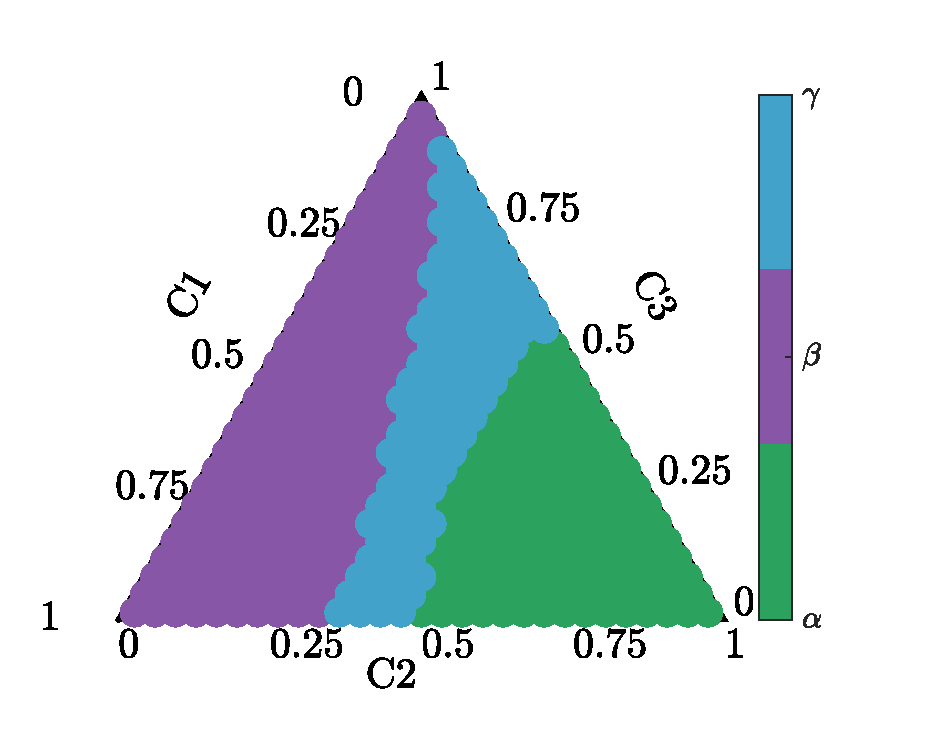
\includegraphics[width=\textwidth]{Chapter-2/figs/Figure1a.eps}
        \caption{}
        \label{origPhase}
    \end{subfigure}
    \quad
    \begin{subfigure}[b]{0.475\textwidth} 
        \centering 
        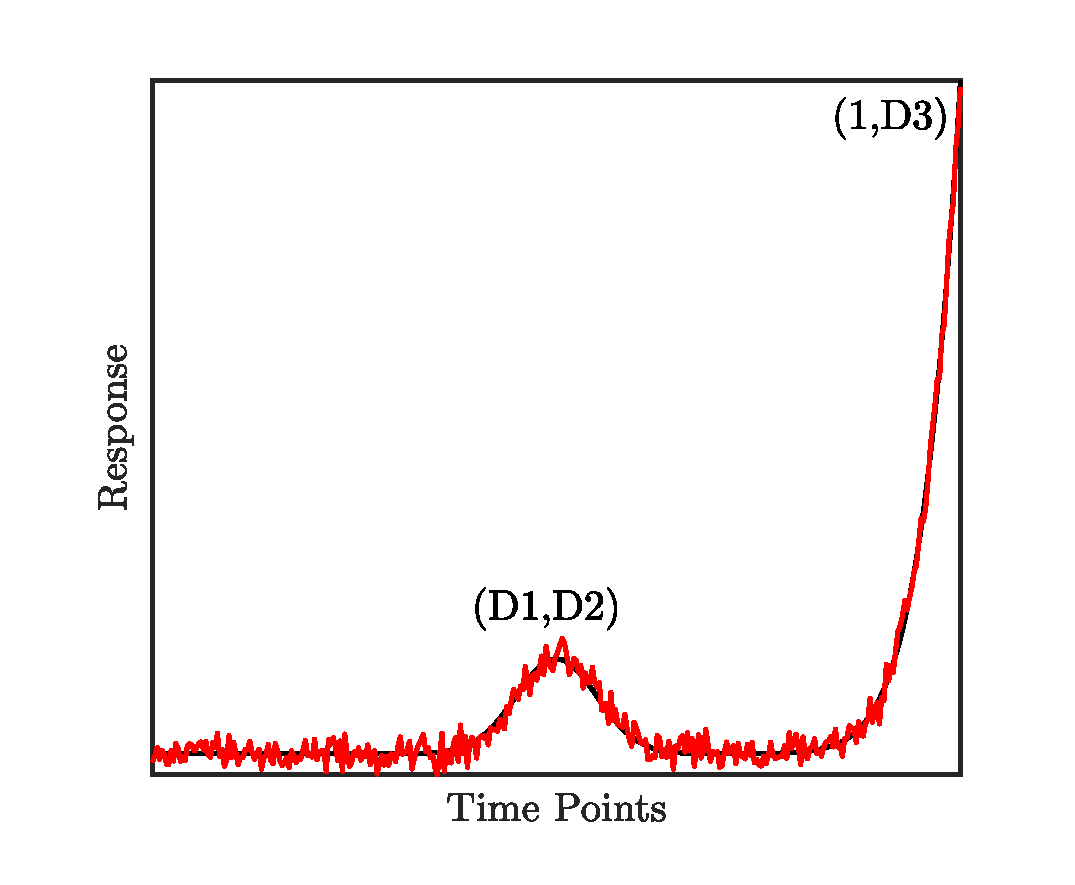
\includegraphics[width=\textwidth]{Chapter-2/figs/Figure1b.eps}
        \caption{}
        \label{sampData} 
    \end{subfigure}
    \vskip\baselineskip
    \caption{(a) Ternary sample with elemental compositions given as C1, C2, C3; partitioned into three known phases. Each color corresponds to one phase. (b) A typical high-dimensional sample response in the synthetic data (red--with Gaussian noise). The degrees of freedom are denoted as D1 (peak position), D2 (peak intensity), D3 (cut-off current)}
    \label{datsExpl}
\end{figure}

\begin{table}[h]
     \centering
\begin{tabular}{|l|l|l|l|l|l|l|}
\hline
& \multicolumn{3}{ |c| }{\textbf{Non-Separable DOFs}} &\multicolumn{3}{ |c| }{\textbf{Separable DOFs}}\\ \hline
Phase in \Cref{origPhase} & D1 & D2 & D3 & D1 & D2 & D3 \\  \hline
\textbf{$\alpha$} & C2+C3 & C3 & 2+C2 & C2+C3 & C3 & 2+C2 \\ 
\textbf{$\beta$} & C2 & C1+C2 & 2+C1 & C2 & C1+C2 & 4+C1 \\ 
\textbf{$\gamma$} & C3 & C1 & 5.0 & C3 & C1 & C1+C3 \\ 
\hline
\end{tabular}
     \caption{DOF variations across each phase for two cases considered in the data sets.}
     \label{DOFsVar}
 \end{table}


\begin{figure}[h]
    \centering
    \begin{subfigure}[b]{0.475\textwidth}
        \centering
        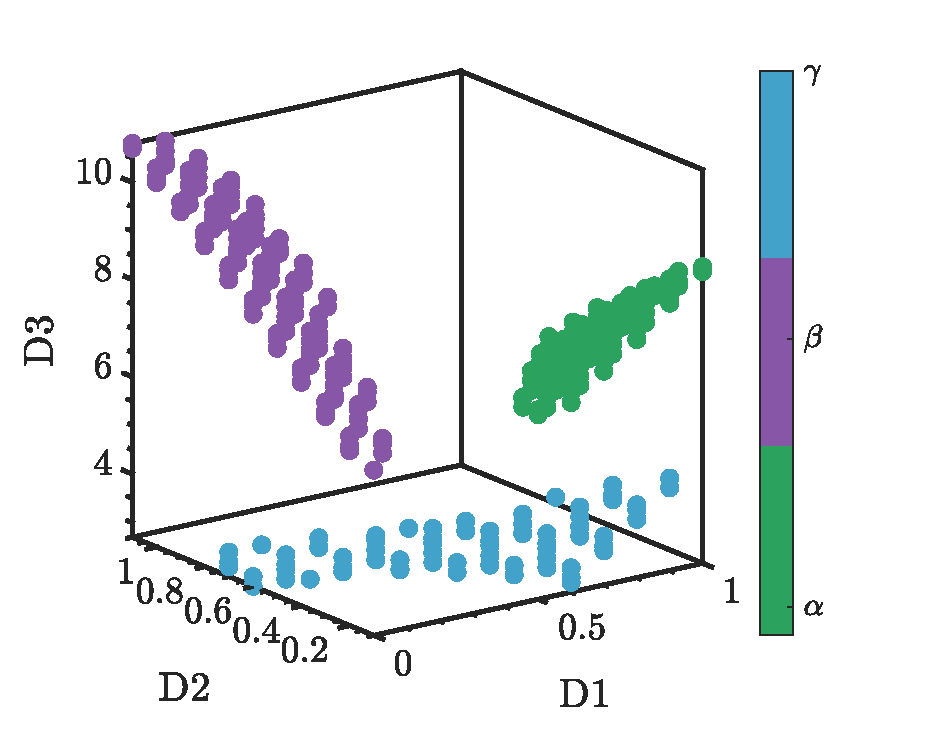
\includegraphics[width=\textwidth]{Chapter-2/figs/figure2a.eps}
        \caption{}
        \label{sepDOFscate}
    \end{subfigure}
    \quad
    \begin{subfigure}[b]{0.475\textwidth} 
        \centering 
        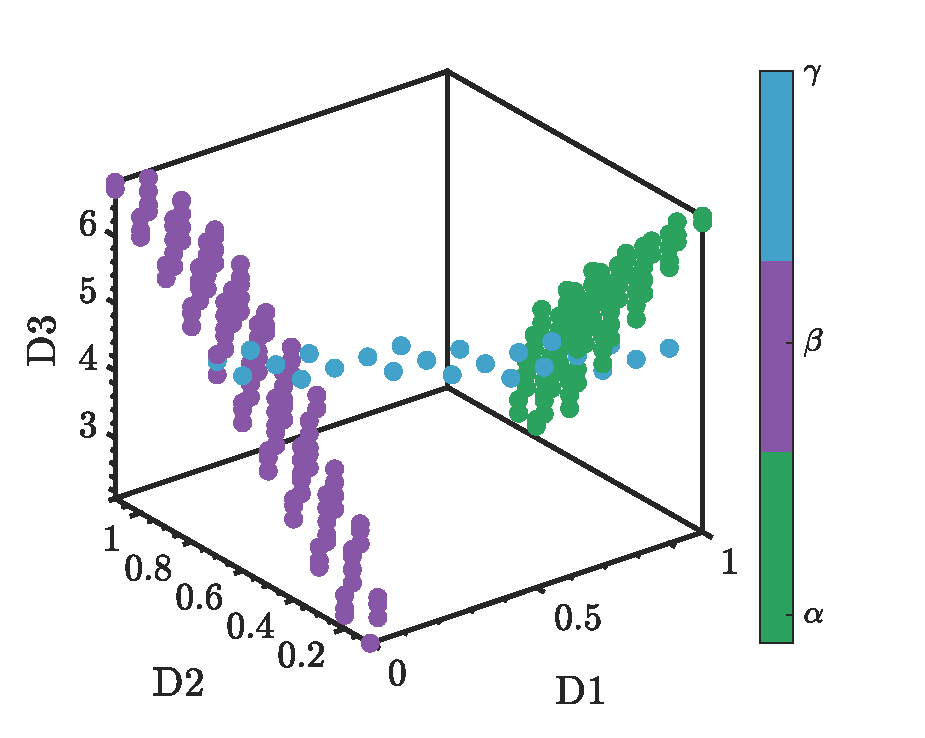
\includegraphics[width=\textwidth]{Chapter-2/figs/figure2b.eps}
        \caption{}
        \label{nonsepDOFscate} 
    \end{subfigure}
    \vskip\baselineskip
    \caption{(a) Phases can be clearly separated in the three dimensional known DOF space (Test cases SET A1,B1) (b) phases can not be separated clearly in three dimensional space (Test cases SET A2,B2)}
    \label{scates}
\end{figure}

% In general, for any given $m$--dimensional HTE data response matrix $X_{m \times n}$ and its corresponding composition matrix $C_{3 \times n}$, its governing $l$--dimensional degrees of freedom matrix $D_{l \times n}$ can be defined using a map $M_{DX}: D_{l\times n} \rightarrow X_{m\times n}$. 
% Learning a compositional phase diagram would require one to partition the map $M_{DX}$ into a set of surjective maps $P_k$ on the data set $\mathcal{D} = (X_{m \times n},C_{3 \times n})$ such that $P_k: \mathcal{C}_{k} \rightarrow \mathcal{X}_{k}$ is continuous in $\mathcal{C}_k \subset C$ for the corresponding $\mathcal{X}_k \subset X$.
% Maps $P_k$, defined above, may result in an irreducible representation (typically a lower dimensional manifold) such that: (1)~the responses form distinct clusters in the lower dimensional embedding ; that is, $P_k$ are distinct  $\forall k $ and $M_{DX}$ is continuous in $C$, or (2)~the responses are overlapping; that is, $P_k$ are distinct $ \forall k $ but $ M_{DX} $ is discontinuous in $C$.
% \begin{figure}[H]
%     \centering
%     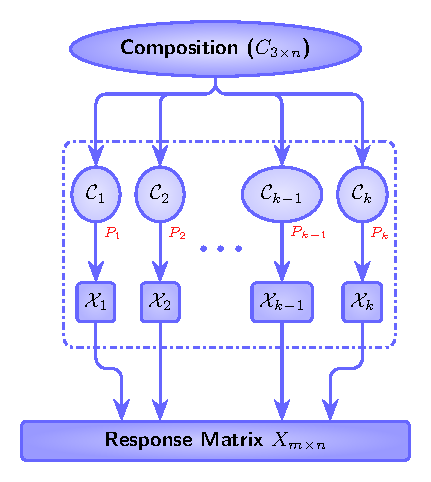
\includegraphics[width=0.5\textwidth, angle=0]{Chapter-2/figs/CompPhaseMap.pdf}
%     \caption{A composition-response map can be seen as a partitioning of the map $M_{DX}$ into various maps $P_k$}
%     \label{compPhaseMap}
% \end{figure}

% Distinct, continuous maps physically signify the dependency of responses entirely on composition (e.g., XRD structural data~\cite{long2007rapid,iwasaki2017comparison}). Presence of a discontinuous map $M_{DX}$ means that at least some responses are not completely governed by composition. In other words, there are at least two samples with similar responses  that are widely separated compositions in the composition space (e.g, cyclic voltammetry data where the overpotential, one of the degrees of freedom of the response, is surjectively mapped to composition with several samples having similar values of overpotential but are very widely separated in composition space~\cite{suram2015generating}). 
%However, we would like to note here that, since composition is not the only variable that governs the response, it is reasonable to assume that for a given phase map $P_k$, some of the governing DOFs of subset of responses $ \mathcal{X}_k$ may not depend on the corresponding composition subset $ \mathcal{C}_k$. Non-existence of map $P_k$ results in an irreducible representation of data (typically a lower dimensional manifold) that does not clearly separate the inherent clusters or phases exist in the data as it has not captured the properties of exact phase map $P_{k}^{E}:D_{l \times n} \rightarrow X_{l \times n}$.%

In this chapter, a data set $\mathcal{D}$ is generated with $k$ phases. Two cases with varying degrees of difficulty are considered.
In each case, three maps for each $k \in \{ 1,2,3 \}$ (see ~\Cref{DOFsVar}) is defined such that the ternary composition space has three inherent non-hyperspherical subsets (e.g., parabolic cuts as shown in~\Cref{origPhase}). 
% Two cases are considered: (1)~the case of separable DOFs that mimics the existence of three distinct surjective phase maps $P_k$, $ \forall k = \{1,2,3\}$ such that $M_{DX}$ is continuous in $C$; and (2)~the case of non-separable DOFs that mimics the discontinuous nature of $M_{DX}$ in $C$ with a set of phase maps such that $P_k$ does not completely represent the respective subset of the $M_{DX}$ map for at least one $k \in \{ 1,2,3 \}$.

The first case, separable DOFs, consists of data points $\mathcal{X}_k$ forming distinct clusters, such as the one shown in~\Cref{sepDOFscate}. 
% This is equivalent to having three distinct maps partitioning the data (i.e., equivalently partitioning the high-dimensional manifold of $X_{m \times n}$) such that mapping is bijective and each composition has a unique response. 
% Formally, $\mathcal{X}_i \bigcap \mathcal{X}_j = \varnothing $, $\forall \mathcal{X}_i, \mathcal{X}_j, i \neq j$, where $\varnothing$ is an empty set. % (Note that since $\bigcap$ is taken for subsets with high dimensional responses as elements, it uses the similarity measure $S$ defined earlier to identify if two responses are same).
% As shown in~\Cref{DOFsVar}, each phase in the separable DOF case is assigned distinct, surjective maps $P_k$ that define DOFs and the corresponding responses $\mathcal{X}_k$.
~\Cref{sepDOFscate} depicts the relationships between DOFs for three maps we used in this work.
The DOFs of each map are marked with a different color. 
In this case, there is no overlap in DOF space between distinct phases.
This clear separation between DOFs makes this data set simpler to analyze with better performance -- as shown in the results section. 
%in the irreducible representation using standard distance metrics since the responses have highly correlated and distinct clusters governed by the corresponding maps $P_k , k = \{ 1,2,3 \}$.
The second case, non-separable DOFs, consists of maps resulting in data points that are not separable on the manifold with DOFs as basis vectors.
% This is equivalent to having three distinct maps $P_1,P_2,P_3$ that divide the data such that $\exists  i, j$ and $\mathcal{X}_i \bigcap \mathcal{X}_j$ is a non-empty set for $ i \neq j \in \{1,2,3\}$.
% ~\Cref{DOFsVar} lists three maps for the non-separable DOF case that we used in this work. 
% Individual phases are named $\alpha$, $\beta$ and $\gamma$. 
% Both phases $\alpha$ and $\beta$ have injective maps $P_{\alpha}$, $P_{\beta}$ that define DOFs where the values of the DOFs do not overlap. 
% This is depicted in~\Cref{nonsepDOFscate}. 
% However, maps $P_{\gamma}$ are defined such that their DOFs overlap with the DOFs defined by two other phases.
% This overlap in DOFs and corresponding data points for $P_{\gamma}$ leads to the case where the inherent phases exist in the data, but their DOFs are not separable, thus making the standard metrics ineffective. (See Supplementary Information for a pictorial representation of the DOFs variation for both types of synthetic data sets.)
With the direct problem stated as above, the goal is to identify the inherent clusters from the high-dimensional data $X$.
% In this work, we aim to learn a metric that closely represents the maps $M_{DX}$ and $P_k$ , where the map $M_{DX}$ represents the inherent clusters in the high-dimensional data $X$, and maps $P_k$ impose constraints relevant to the compositional continuity in $C$. 
% This continuity constraint motivates the similarity measure that combines similarity in response space as well as the nearest neighborhood in the corresponding composition space.
%We generate two sets of synthetic data with varying degree of complexity.
%In both cases, we generate response curves such that ternary composition diagram is divided into three subsets (phases) with three distinct maps: $P_k: C_{3\times n} \rightarrow D_{3 \times n}$ where $k=1,2,3 $ for each of the three phases shown in ~\Cref{origPhase}.

\begin{table}[h]
     \centering
\begin{tabular}{ |l|l| }
  \hline
  \multicolumn{2}{|c|}{Test data sets} \\
  \hline
  SET A1 & Separable DOFs \\
  SET A2 & Non-Separable DOFs \\
  SET B1 & Separable DOFs, Noisy data $\sim \mathcal{N}(0,0.1)$ \\
  SET B2 & Non-Separable DOFs, Noisy data $\sim \mathcal{N}(0,0.1)$ \\
  \hline
\end{tabular}
    \captionsetup{justification=centering}
     \caption{Description of data sets used for evaluation. Gaussian noise is added with variance approximately 10 \% of the peak intensity}
     \label{datasets}
 \end{table}
 
\subsection{Comparison between several distance measures}
To learn a metric for data matrix $X$ using the framework introduced earlier, each element in the ternary space is considered as a task. 
For a ternary system, three tasks are considered. 
In each task, we define a class by sorting the data points based on corresponding element content and sequentially categorizing the data point.
The generated data set consists of 435 data points, giving four classes for a given task (each class consists of 100 points, with the remaining 35 points in the last class added to the penultimate class).
The procedure is repeated for the remaining tasks, giving three sets of incompatible labels.

We will now compare distance metric learned in the MT-LMNN framework (with tasks and classes defined as above) with other commonly used distance measures such as Euclidean, cosine metrics, correlation, dynamic time warping (DTW), etc. 
% \begin{itemize}
%     \item Hierarchical clustering algorithm (HCA) with three different linkage options (average, complete, single) with varying number of clusters
%     \item  Spectral clustering method\cite{ng2002spectral,zelnik2005self} to partition the graph generated on the composition data with weights defined by a similarity measure. The graph is generated using either the 10-nearest neighbor algorithm or Delaunay tessellation. Local scaling of similarity measure mentioned in~\cite{zelnik2005self} is varied from two to six along with a varying number of clusters.
% \end{itemize}
For each metric, we use two sets of clustering algorithms (detailed below), with various settings possible:
\begin{itemize}
    \item Hierarchical clustering algorithm (HCA) with three different linkage options (average, complete, single) with varying numbers of clusters(for example,~\(\{k_0-1,k_0,k_0+1\}\) where $k_0$ is actual number of clusters).
    \item  Spectral clustering method\cite{ng2002spectral,zelnik2005self} to partition the graph generated on the composition data with weights defined by a similarity measure. The graph is generated using either the 10-nearest neighbor algorithm or Delaunay tessellation. Local scaling of similarity measure mentioned in~\cite{zelnik2005self} is varied from two to six along with a varying number of clusters (for example,~\(\{k_0-1,k_0,k_0+1\}\) where $k_0$ is actual number of clusters).
\end{itemize}

Clustering is selected as a indirect way of evaluating the performance (and importance) of a distance measure. In general, clustering aims to find homogeneous subgroups such that data points in each cluster are similar according to the similarity measure.
If the distance measure can capture the key features defining the similarity (in the context of the output quantity), the subgroups can be separated, and clustering will provide insight into data.
If informative features are selected, clustering is an appropriate technique to find subgroups in the input data.

The accuracy of clustering is evaluated based on the F-measure calculated using~\Cref{eq41}:
\begin{equation}\label{eq41}
    \begin{aligned}
    & F = \sum_{i=1}^{k} \frac{\abs{A_i}}{N} \underset{j}{\text{max}}  \frac{2R_{ij}P_{ij}}{R_{ij}+P_{ij}}\\
    & P_{ij}=\frac{\abs{A_i\cap B_j}}{\abs{B_j}}\\
    & R_{ij}=\frac{\abs{A_i\cap B_j}}{\abs{A_j}}
    \end{aligned}
\end{equation}
where $\abs{\mathcal{A}}$ returns the number of elements in the vector $\mathcal{A}$; $N$ is the total number of samples; $P$ is the precision and $R$ is the recall.
To calculate the F-measure, pre-defined labels ($A_i$) for phase $i$ are used to compare with labels from the graph partitioning $B_j$.  
Intuitively, the F-measure evaluates if a group of samples are clustered the same as the known clusters (or phases). 
If all samples were classified correctly, the F-measure equals one. 
The lower the value of this measure, the poorer the classification performance. We report the mean value and standard deviation of the F-measure from various clustering settings mentioned above as the stochastic performance measure of the metric on any given data set. This is performed to alleviate any inconsistencies in the F-measure that may arise from various clustering settings. The standard deviation in stochastic F-measures quantifies the consistency (or stability) of clustering for a given distance measure.  This way of looking at the data helps to quantify the effect of the metric on learning a response map.

%{\color{red}In general, the clustering performance is difficult to evaluate~\cite{caruana2006meta}. Several approaches (including F-measure) are being used with their strengths and weaknesses.We list alternative clustering performance evaluation in the Supplementary Information. However, F-measure is the most widely used and accepted by the community~\cite{manning2010introduction}. }

\begin{figure}[h]
    \centering
    \begin{subfigure}[b]{0.475\textwidth}
        \centering
        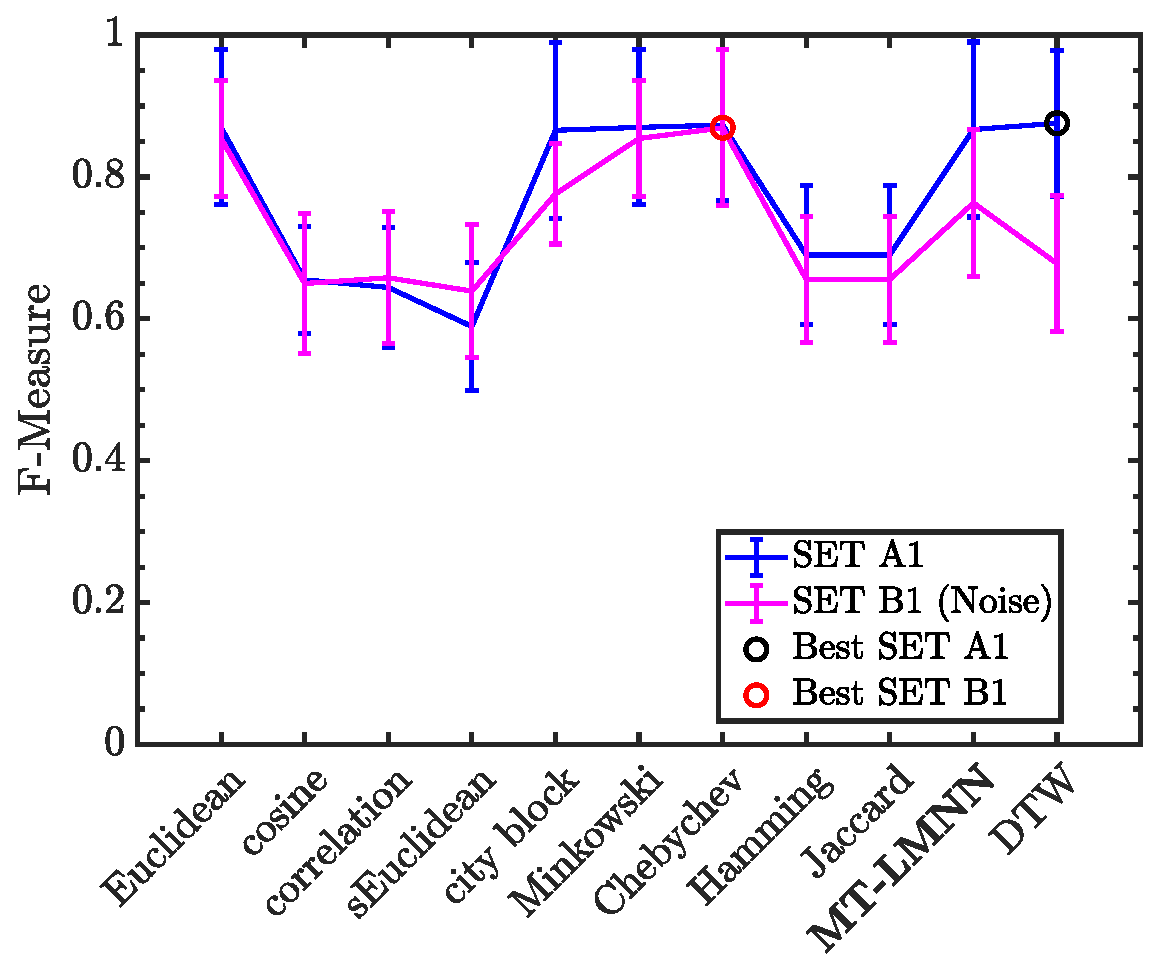
\includegraphics[width=\textwidth]{Chapter-2/figs/SD.eps}
        \caption{Separable DOFs}
        \label{errSD}
    \end{subfigure}
    \quad
    \begin{subfigure}[b]{0.475\textwidth} 
        \centering 
        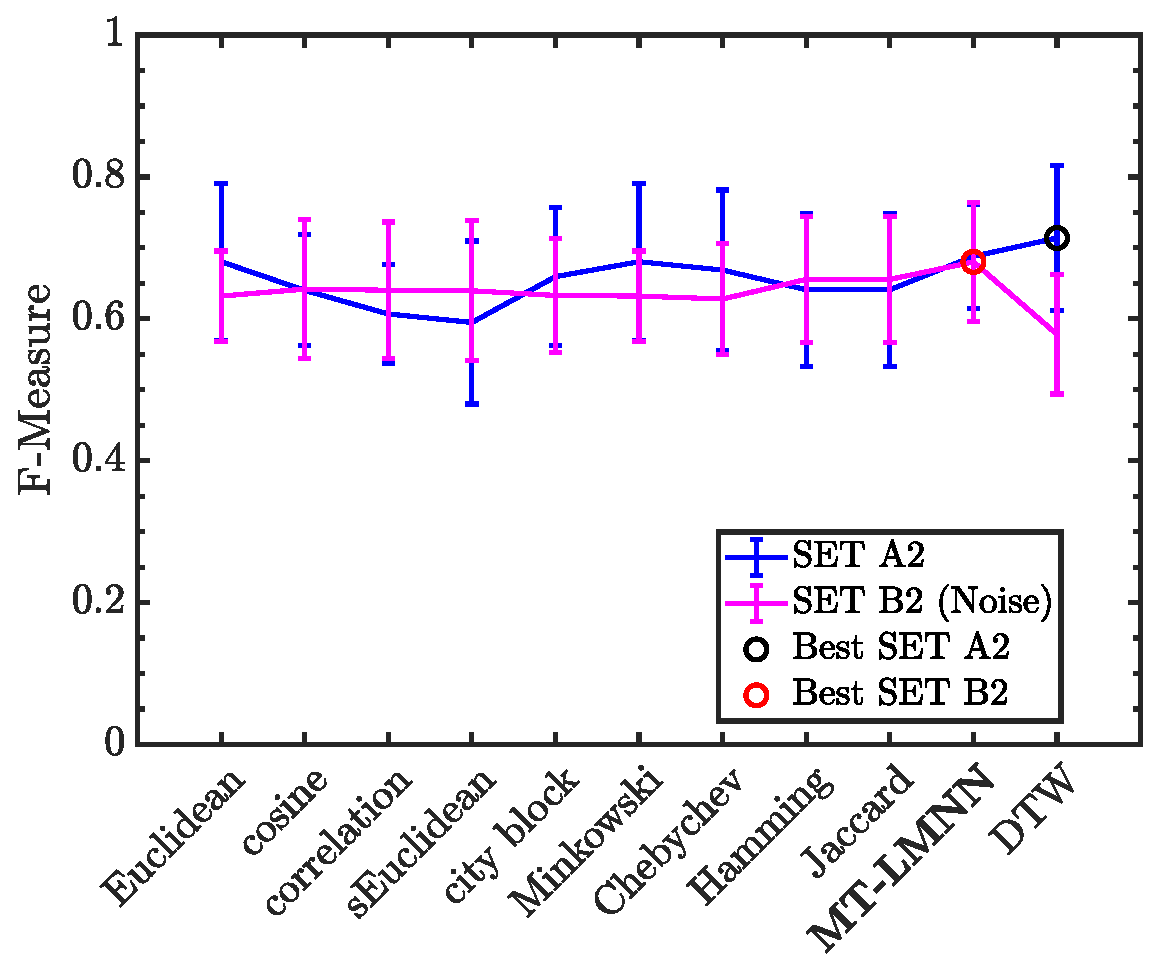
\includegraphics[width=\textwidth]{Chapter-2/figs/NSD.eps}
        \caption{Non-Separable DOFs}
        \label{errNSD} 
    \end{subfigure}
    \vskip\baselineskip
    \caption{F-measure statistics suggest that the similarity measure learned using MT-LMNN is at least as good as the best similarity measure obtained from exhaustive search over several metrics in all cases. We used Euclidean, cosine, correlation, standardized Euclidean (sEuclidean), city block, Minkowski, Chebychev, Hamming, Jaccard and dynamic time warping (DTW)  for an exhaustive similarity measure search.~\Cref{errSD} corresponds to separable DOFs case,~\Cref{errNSD} corresponds to non-separable DOFs case as described in the text.}
    \label{errorsDataNoise}
\end{figure}

\Cref{errorsDataNoise} contains the comparison between the performance of several distances and the approach taken in this work, MT-LMNN. 
The comparison is performed for two data sets with separable (A1) and non-separable DOFs (A2). 
Two additional data sets are analyzed with the noise added (data sets annotated with B - see Table~\ref{datasets}). To calculate F-measure statistics, we vary the number of clusters from two to three for all the cluster settings mentioned above.  

Our analysis shows that the similarity measure learned using MT-LMNN augments the ability to find regions with high composition-response correlation.
MT-LMNN is at least as good as the best distance measure obtained from an exhaustive search sometimes outperforming the complex, more sophisticated dynamic time warping (DTW). % Unlike DTW (which has the best stochastic F-measure in SET A1, A2 ), MT-LMNN is insensitive to the effect of noise (SET B2). %
We also note that analysis of each of the four data sets considered in~\Cref{datasets} resulted in four different measures as the best. However, MT-LMNN's performance was comparable to the best distance measure for SET A1, A2 (i.e., DTW) while producing the best accuracy in SET B2 (complex data set of the four). This also highlights the ability of MT-LMNN to quantify similarity automatically without any expert knowledge about the data that is required to select DTW or Chebychev.

We attribute the excellent performance of MT-LMNN to the local learning characteristics. 
The metric is learned in a small local neighborhood of each data point (determined by its classes). Learning a metric locally in a small neighborhood defined by the design space variable helps the clustering method to identify phases where the data responses are highly correlated but undergo systematic variation with the design space.
Results presented in this work demonstrate that this approach is robust even for the variation in degrees of freedom over a large range of composition. 

We would like to note that although the F-measure is widely used and accepted by the community~\cite{manning2010introduction}, it may not represent a pure performance of clustering~\cite{powers2015f}. However, there is no other good alternative to address the performance of clustering. 
To check if different conclusion is reached for other clustering performance measures, we performed the analogous analysis for other measures. 
We performed the analysis for four other performance measures: the adjusted rand index, the adjusted mutual information, the normalized mutual  information and Fowlkes-Mallows scores. 
Interestingly, regardless of selected performance evaluation measure, we reached the same observation. 
We additionally performed the one-sided paired t-test between MT-LMNN and the best metric.
We designed the hypothesis test to classify how similar (or dissimilar) are two metrics in terms of any given clustering performance measure distribution over clustering settings that are varied.  
Our additional analysis reiterates the main conclusion that MT-LMNN is at least as good as the best distance measure obtained from the exhaustive search.

\section{Results of t-test for synthetic CV data sets}
In this section, statistical comparison of various distance functions is performed with the following protocol. (1)~For each of the clustering settings and distance measure, we record the predicted labels. (2)~Using these labels and true labels, we compute four different clustering performance measures (ARI, AMI, NMI, FWS) from scikit-learn python library~\cite{sklearn}. 
The four performance measures:~(a)~the adjusted rand index (ARI)-- which measures the similarity of our predicted labels  with  true  labels  ignoring permutations with a normalized chance~\cite{santos2009use}; mutual information,-- which measures agreement between the true and predicted labels ignoring permutations, with two variants being used~(b)~adjusted mutual information (AMI), which is normalized against chance~\cite{hubert1985comparing};~(c)~normalized  mutual  information (NMI),  which is mutual information normalized  by the product  of  entropies  of predicted and true labels~\cite{strehl2002cluster,vinh2010information}; and ~(d)~Fowlkes-Mallows scores (FWS)~\cite{fowlkes1983method}.
(3)~For each distance and each performance measure, we compute the mean value of performance measures - see Table~\ref{ttest_setb2} for the example summary. Next, we select a distance measure with the highest mean to be the best for a given performance measure.
We then perform a one-sided paired t-test between MT-LMNN and the best distance measure. 
We define the Null hypothesis for any given performance measure to be:~\texttt{MT-LMNN is similar to the best distance measure}.
The hypothesis test described above is designed to classify how similar (or dissimilar) are two distance measures in terms of any given clustering performance measure distribution over clustering settings that are varied.  

We record the hypothesis test result $h$ obtained using the one-sided paired t-test (with a significance level of 0.01). 
A value of \(h=0\) signifies that the t-test failed to reject the null hypothesis while a value of \(h=1\) signifies the rejection of our null hypothesis.
Table~\ref{ttest_cv} summarizes the results from the t-test. If MT-LMNN is the best distance, we count number of performance measure for which it is the best. For example, MT-LMNN is the best distance according to all 4 performance measures for data set SET B1 (see~\Cref{ttest_setb1}). Similarly, we count number of tests for which the hypothesis was rejected and failed to be rejected.  

Here, we show the results for the CV data sets considered above.  \Cref{ttest_seta1,ttest_seta2,ttest_setb1,ttest_setb2} report the mean value of four different performance measures considered for SET A1 and B2. 
%As a reminder, these sets correspond to synthetic CV data sets with separable and non-separable degrees of freedom with noise, respectively. 
The distance measure with the highest mean is marked using bold text and the h-value from the paired one-sided t-test is reported.

~\Cref{ttest_cv} displays the results for all four CV datasets. Specifically, we present the number of performance measures for which MT-LMNN came out to be best, failed to reject and reject. Please note that we focus only on cases when a measure other than MT-LMNN is the best (SET B1). 
In the case of SET A2, for all four performance measures the Null hypothesis failed to be rejected. As a reminder, the Null hypothesis states: MT-LMNN is similar to the best distance measure. Only for SET A2, MT-LMNN is rejected to be performing comparable to the best distance functions (i.e., Chebychev).


In summary, regardless of the performance measure used, MT-LMNN is at least as good as the best distance measure obtained from the exhaustive search. 
In many cases, MT-LMNN outperforms the standard similarity measure, including more sophisticated and computationally demanding distance measures such as dynamic time warping (DTW). 

\begin{table}[h]
     \centering
    \begin{tabular}{ |c|c|c|c| }
      \hline
      Data set & Best & Failed to reject & Rejected \\
      \hline
      SET A1 & 0 & 4 & 0 \\
      \hline
      SET A2 & 0 & 0 & 4 \\
      \hline
      SET B1 & 4 & 0 & 0 \\
      \hline
      SET B2 & 0 & 3 & 1 \\
      \hline
    \end{tabular}
        \captionsetup{justification=centering}
         \caption{The number of performance measures MT-LMNN has been classified into each of the three categories--best, failed to reject, reject--for the four synthetic data sets introduced earlier.}
         \label{ttest_cv}
 \end{table}
 
\begin{table}[h]
     \centering
    \begin{tabular}{ |c|c|c|c|c| }
      \hline
    Measure    & 	 AMI &	 ARI &	 FMS &	 NMI \\
    \hline
    Chebychev & 	 0.76 &	 0.76 &	 0.87 &	0.85 \\
    city block  &	 0.74 &	 0.75 &	 0.87 &	0.83  \\
    correlation &	 0.24 	& 0.28 &	 0.62 &	0.29 \\
    cosine    & 	 0.33 &	 0.35 &	 0.65 &	0.38 \\
    Euclidean & 	 \textbf{0.76} 	& \textbf{0.76} 	& 0.87 &	\textbf{0.85} \\
    Hamming    &	 0.33 &	 0.36 &	 0.66 &	0.39 \\
    Jaccard   & 	 0.33 &	 0.36 &	 0.66 &	0.39 \\
    Minkowski & 	 0.76 &	 0.76 &	 0.87 &	0.85 \\
    DTW       & 	 0.73 &	 0.77 &	 \textbf{0.88} &	0.81 \\
    MT-LMNN  &  	 0.76 &	 0.76 	& 0.87 &	0.85 \\
    sEuclidean &	 0.21 &	 0.21 	& 0.62 &	0.27 \\
    \hline
    $h$   &  	 0.00 &	 0.00 &	 0.00 &	0.00 \\
    \hline
    \end{tabular}
    \captionsetup{justification=centering}
     \caption{Mean value of four different performance measures for all the distance measures studied for SET A1 (synthetic CV data sets with separable DOFs and no noise). The best distance measures are highlighted. For this data set, MT-LMNN is failed to reject for all the performance measure as its performance is comparable to the best performing measure. }
     \label{ttest_seta1}
 \end{table}
 
\begin{table}[h]
     \centering
    \begin{tabular}{ |c|c|c|c|c| }
      \hline
    Measure    & 	 AMI &	 ARI &	 FMS &	 NMI \\
    \hline
    Chebychev  &	 \textbf{0.75} 	& \textbf{0.74} &	 \textbf{0.85} &	\textbf{0.84} \\
    city block  	& 0.56 	& 0.54 &	 0.72 &	0.63 \\
    correlation &	 0.29 &	 0.30 &	 0.59 &	0.33 \\
    cosine     &	 0.28 	& 0.30 	& 0.59& 	0.33 \\
    Euclidean & 	 0.72 &	 0.72 &	 0.84 &	0.81 \\
    Hamming  &  	 0.25 	& 0.25 &	 0.58 &	0.28 \\
    Jaccard   & 	 0.25 &	 0.25 &	 0.58 &	0.28 \\
    Minkowski  &	 0.72 	& 0.72 &	 0.84 &	0.81 \\
    DTW      &  	 0.54 &	 0.54 &	 0.74 &	0.62 \\
    MT-LMNN   & 	 0.54 &	 0.53 &	 0.71 &	0.61 \\
    sEuclidean &	 0.30 &	 0.31 &	 0.60 &	0.36 \\
    \hline
    $h$   &  	 1.00 &	 1.00 &	 1.00 &	1.00 \\
    \hline
    \end{tabular}
    \captionsetup{justification=centering}
     \caption{Mean value of four different performance measures for all the distance measure studied for SET A2(synthetic CV data sets with not-separable DOFs and no noise). For this data set, Chebychev is selected as the best distance measure for all of the performance measures used and MT-LMNN is rejected to be performing comparable to Chebychev.}
     \label{ttest_seta2}
 \end{table}
 
\begin{table}[h]
\centering
    \begin{tabular}{ |c|c|c|c|c| }
      \hline
    Measure    & 	 AMI &	 ARI &	 FMS &	 NMI \\
    \hline
    Chebychev  &	 0.36 &	 0.36 &	 0.64 &	0.42 \\
    city block  &	 0.32 &	 0.34 &	 0.65 &	0.38 \\
    correlation &	 0.17 &	 0.16 &	 0.58 &	0.24 \\
    cosine   &  	 0.23 &	 0.25 &	 0.62 &	0.28 \\
    Euclidean  &	 0.41 &	 0.40 &	 0.66 &	0.47 \\
    Hamming  &  	 0.25 &	 0.27 &	 0.60 &	0.28 \\
    Jaccard   & 	 0.25 &	 0.27 &	 0.60& 	0.28 \\
    Minkowski & 	 0.41 &	 0.40 &	 0.66& 	0.47 \\
    DTW       & 	 0.38& 	 0.38 &	 0.64 &	0.43 \\
    MT-LMNN   & 	\textbf{ 0.41} &	 \textbf{0.44} &	 \textbf{0.68} &	\textbf{0.47} \\
    sEuclidean &	 0.22 &	 0.21 &	 0.62 &	0.28 \\
    \hline
    \end{tabular}
    \captionsetup{justification=centering}
     \caption{Mean value of four different performance measures for all the distance measure studied for SET B1(synthetic CV data sets with not-separable DOFs with noise). For this test case MT-LMNN is adjudged the best distance measure for all of the performance measures considered.}
     \label{ttest_setb1}
 \end{table}
 
\begin{table}[h]
     \centering
\begin{tabular}{ |c|c|c|c|c| }
  \hline
Measure    & 	 AMI &	 ARI &	 FMS &	 NMI \\
\hline
Chebychev & 	 0.27 &	 0.24 	& 0.54 &	0.31 \\
city block  &	 0.25 &	 0.24 &	 0.55 &	0.29 \\
correlation &	 0.26 &	 0.26 &	 0.57 &	0.30 \\
cosine    & 	 0.27 &	 0.27 &	 0.58 &	0.31 \\
Euclidean  	& 0.27 	& 0.24 	& 0.54 &	0.31 \\
Hamming    &	 0.25 &	 0.25 &	 0.58 &	0.28 \\
Jaccard   & 	 0.25 &	 0.25 &	 0.58 &	0.28 \\
Minkowski  &	 0.27 &	 0.24 &	 0.54 &	0.31 \\
DTW       & 	 \textbf{0.32} &	 \textbf{0.32} &	 0.60 &	\textbf{0.37} \\
MT-LMNN   & 	 0.25 &	 0.22 &	 0.60 &	0.31 \\
sEuclidean &	 0.29 &	 0.30 &	 \textbf{0.60} &	0.34 \\
\hline
$h$ &    	 0.00& 	 1.00 &	 0.00 &	0.00 \\
\hline
\end{tabular}
    \captionsetup{justification=centering}
     \caption{Mean value of four different performance measures for all the distance measure studied for SET B2 (synthetic CV data sets with Not-separable DOFs with a Gaussian noise). Note MT-LMNN performance is comparable to more sophisticated DTW.}
     \label{ttest_setb2}
 \end{table}


%%%%%%%%%%%%%%%%%%%%%%%%%%%%%%%%%%%%%%%%%%%%%%%%%%%%%%%%%%%%%%%%%%%%%%%%%%%%%%%%%%%%%%%%%%%%%%%%%%%%%%%%%%
\subsection{Phase diagram construction from XRD measurements}

\subsubsection{Data description}
In this section, we use the labeled data sets by Long et al. \cite{long2007rapid}. 
This data set corresponds to the ternary library of Fe-Pd-Ga prepared by elemental sputtering. 
The data set contains 278 diffractograms (each of 1616 dimensions), and the corresponding composition map. 
The diffraction patterns are collected in 1D intensity versus 2$\theta$ diffractograms. 
The labeled data from \cite{long2007rapid} is available as sample data sets with Gphase~\cite{xiong2017automated} -- a software for clustering analysis using graph partition of high-throughput experimental data.
This data set was used by Iwasaki et al. in\cite{iwasaki2017comparison} to compare various distance measures and their performance to determine the phase diagrams of this system. 


\subsubsection{Comparison between several distance measures}
Similar to the previous case study with model cyclic voltammetry data, we compare the performance of several similarity measures against MT-LMNN.
The metric is learned on the data matrix $X_{1616\times278}$ with tasks and classes defined using the procedure briefed for synthetic data with a segmentation after every 75th sorted data point under a given task. 
To balance the data dimensions, we reduce the dimensionality of $X$ by projecting the data onto its leading principal components sufficient to capture \(100\%\) variance. 
As an outcome, the dimensionality of the input data is reduced from 1616 to 191. 


We compute the stochastic F-measure for each of the distance measures using the procedure briefed in the previous section with a varying number of clusters from five to seven. 
To compute the F-measure, we used labels from~\cite{long2007rapid}.
A summary of our results is depicted in~\Cref{errorsFePdGa}. 
The phase diagram reported in~\cite{long2007rapid} has six clusters and they can be seen in~\Cref{refFePdGa}, with each cluster being annotated with a single color and a unique numeric index.
\Cref{errorsFePdGa} shows the stochastic F-measure for each of the distance measures considered with the best performing measure highlighted in the black circle and our method in the red circle. 
It can be observed that performance of MT-LMNN is as good as the best performing distance measure. 


Although the similarity measure computed using correlation has the best performance in terms of F-measure, it splits the single phase with a systematic variation in peak position (Cluster 4 in~\Cref{refFePdGa}) into two clusters (1 and 4 in~\Cref{FePdGaCorr}).
In contrast, the MT-LMNN--based similarity measure identifies the phase with peak shift to be a single cluster (4 in \Cref{FePdGaMLPD}). 
This example demonstrates that in this case the learned distance measure is shift resilient.  This is of high importance as shift resiliency is one of the critical issues stated for XRD phase identification~\cite{iwasaki2017comparison,hattrick2016perspective}. The split region near the Fe-lean region in~\Cref{FePdGaMLPD} is an interesting case and requires further study. Recently~\cite{bunn2016semi} it has been reported that the Fe-Pd-Ga data set has two unknown phases near the Fe lean end (Figure 3 a,b in~\cite{bunn2016semi}). It is possible that this split region is linked to these unknown phases.

\begin{figure}[h]
    \centering
    \begin{subfigure}[b]{0.475\textwidth} 
        \centering 
        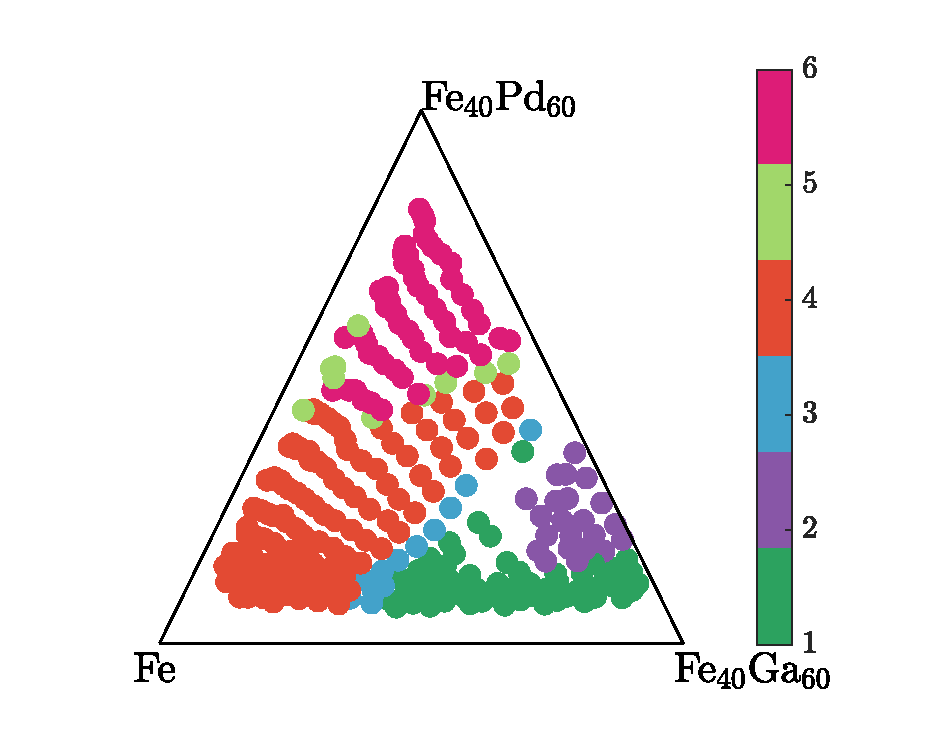
\includegraphics[width=1\textwidth]{Chapter-2/figs/fig5a.eps}
        \caption{Phase diagram reported in \cite{long2007rapid}}
        \label{refFePdGa}
    \end{subfigure}
    \quad
        \begin{subfigure}[b]{0.475\textwidth} 
        \centering 
        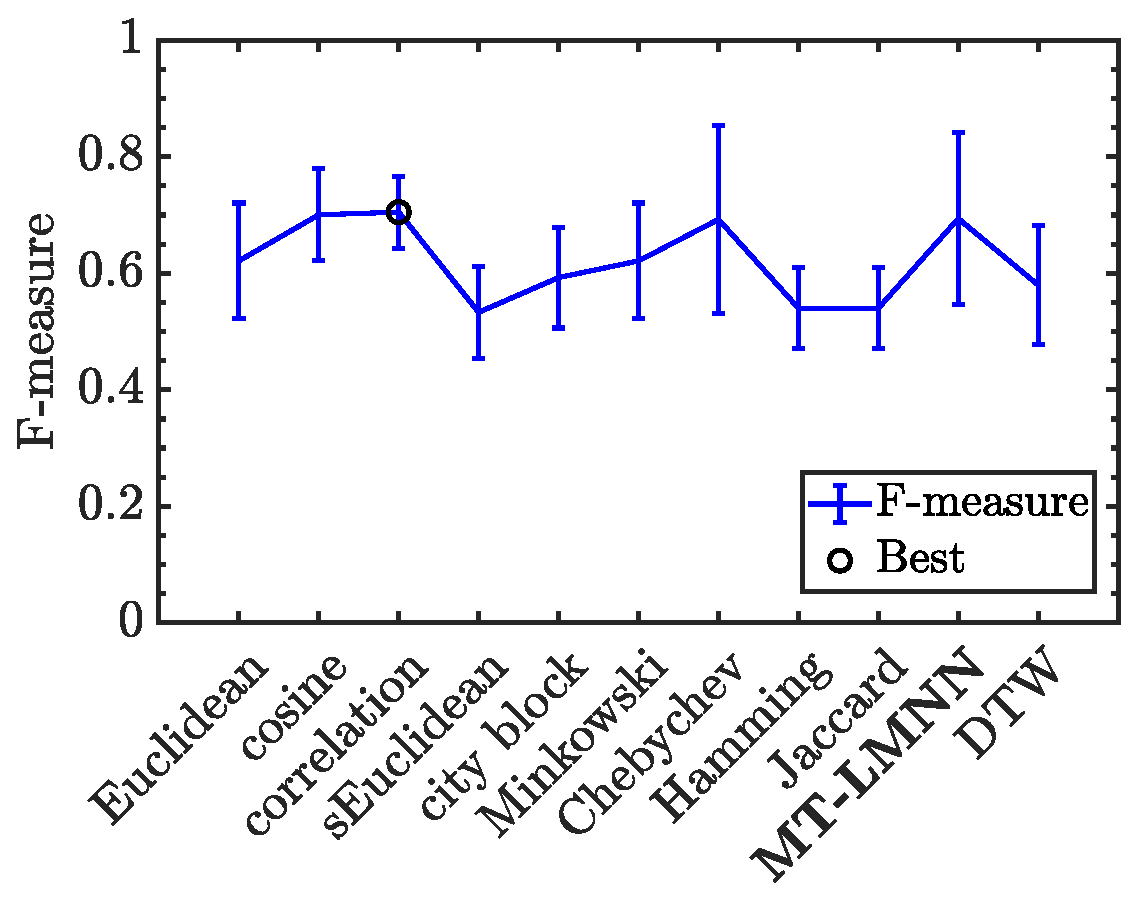
\includegraphics[width=1\textwidth]{Chapter-2/figs/fig5b.eps}
        \caption{F-measure statistics}
        \label{errorsFePdGa}
    \end{subfigure}
    \quad
    \vskip\baselineskip
        \begin{subfigure}[b]{0.475\textwidth} 
        \centering 
        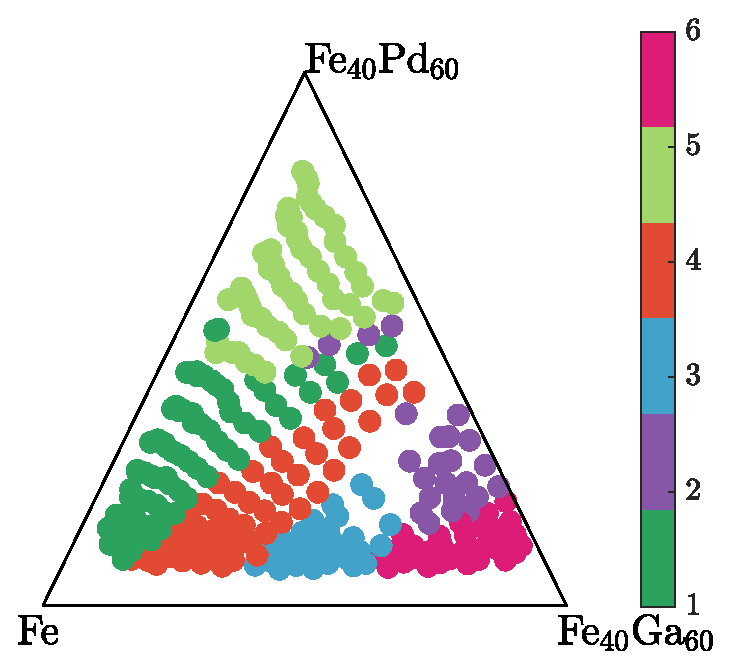
\includegraphics[width=0.8\textwidth]{Chapter-2/figs/fig5c.eps}
        \caption{Phase diagram using correlation}
        \label{FePdGaCorr}
    \end{subfigure}
    \quad
    \begin{subfigure}[b]{0.475\textwidth} 
        \centering 
        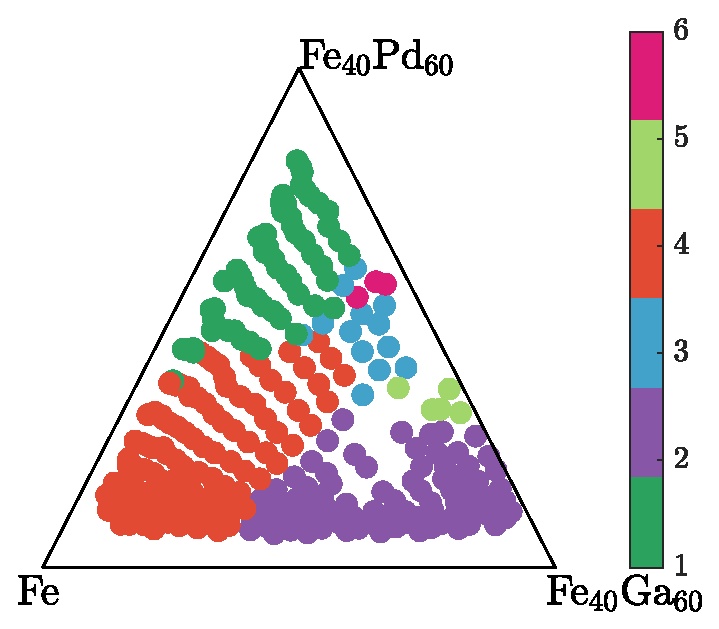
\includegraphics[width=0.8\textwidth]{Chapter-2/figs/fig5d.eps}
        \caption{Phase diagram using MTML}
        \label{FePdGaMLPD}
    \end{subfigure}
\caption{Comparison of phase diagram deduced using various similarity measure. \Cref{FePdGaCorr,FePdGaMLPD} depict the representative phase diagrams (most frequent or stable for among various clustering settings/parameters used for the true number of clusters).}
    \label{FePdGa}
\end{figure}
\section{Conclusions}
In this chapter, we introduced a distance measure learning approach into the data analytics for compositional libraries. 
A metric was learned from the data using the composition information about the design space. 
This is in contrast to the exhaustive search for a suitable distance measure.
Two case studies consisting of model cyclic voltammetry and experimental XRD responses as high-dimensional signals are presented and evaluated using a variety of statistical tests.
We showed that our method has the ability to identify regions in the design space where a systematic variation in design variable gives rise to systematic variation in response. 
Using a model electrochemistry data, we showed that a distance measure learned using our approach is at least as good as the metric chosen using an exhaustive search.
Through various test cases, we have shown that learning a similarity measure using MT-LMNN has the ability to automatically quantify the similarity measure for any given data set. This makes MT-LMNN a better alternative to an exhaustive search of complex and data specific metrics as well as a promising approach for automated distance learning for compositional libraries. 
